\documentclass[10pt,a4paper]{article}

% ── Packages ────────────────────────────────────────────────────────────────
\usepackage[utf8]{inputenc}
\usepackage[T1]{fontenc}
\usepackage[french]{babel}
\usepackage[margin=0.45in]{geometry}
\usepackage{enumitem}
\usepackage{titlesec}
\usepackage{xcolor}
\usepackage{fontawesome5}
\usepackage{hyperref}
\usepackage{tabularx}
\usepackage{array}
\usepackage{graphicx}
\usepackage{tikz}

% ── Couleurs (alignées au portfolio HUD) ────────────────────────────────────
\definecolor{accent}{HTML}{0891B2}
\definecolor{ink}{HTML}{111827}
\definecolor{muted}{HTML}{4B5563}

% ── Hyperliens ──────────────────────────────────────────────────────────────
\hypersetup{
    colorlinks=true,
    urlcolor=accent,
    linkcolor=accent
}

% ── Typographie \& mise en page ─────────────────────────────────────────────
\pagestyle{empty}
\setlength{\parskip}{0pt}
\setlength{\parindent}{0pt}
\raggedbottom

\titleformat{\section}
  {\large\bfseries\color{accent}}
  {}{0em}{}[\vspace{1pt}{\color{accent}\titlerule}]
\titlespacing*{\section}{0pt}{5pt}{2.5pt}

\setlist[itemize]{
    leftmargin=1.1em,
    topsep=0.5pt,
    itemsep=1.0pt,
    parsep=0pt,
    label=\textcolor{accent}{\textbullet}
}

% ── Helpers ─────────────────────────────────────────────────────────────────
\newcommand{\cvname}[1]{{\LARGE\bfseries\color{ink}#1}}
\newcommand{\cvtitle}[1]{{\normalsize\color{muted}#1}}
\newcommand{\cvmeta}[1]{{\footnotesize\color{muted}#1}}
\newcommand{\role}[2]{\textbf{#1}\hfill\textit{\color{muted}#2}\\}
\newcommand{\org}[1]{\textit{#1}\\[0.5pt]}

% Photo de profil circulaire (Overleaf : garder profile-photo.jpg à côté de ce .tex)
\newcommand{\profilephoto}{%
    \begin{tikzpicture}
        \clip (0,0) circle (1.15cm);
        \node[anchor=center] at (0,0) {%
            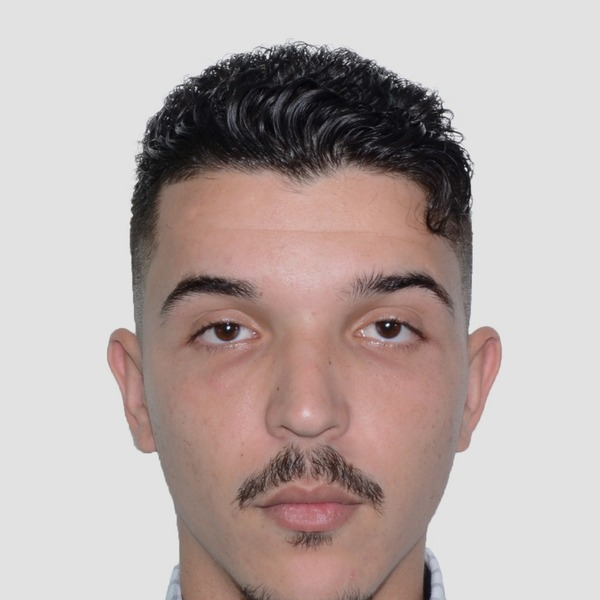
\includegraphics[width=2.3cm]{profile-photo.jpg}%
        };
        \draw[accent, line width=1.2pt] (0,0) circle (1.15cm);
    \end{tikzpicture}%
}

\begin{document}
\normalsize
\setlength{\tabcolsep}{0pt}

% ── En-tête avec photo ──────────────────────────────────────────────────────
\noindent
\begin{minipage}[c]{0.17\textwidth}
    \centering
    \profilephoto
\end{minipage}%
\hfill
\begin{minipage}[c]{0.80\textwidth}
    \cvname{Hamza Bouktitiya}\\[2pt]
    \cvtitle{Ingénieur en Intelligence Artificielle \textbullet\ Doctorant}\\[4pt]
    \cvmeta{%
        \faMapMarker*\ Kenitra, Maroc
        \quad\textbullet\quad
        \faPhone*\ +212~688~679~653
        \quad\textbullet\quad
        \faEnvelope*\ \href{mailto:bouktitiya.hamza.post@gmail.com}{bouktitiya.hamza.post@gmail.com}
    }\\[2pt]
    \cvmeta{%
        \faLinkedin*\ \href{https://www.linkedin.com/in/hamza-bouktitiya-604471253/}{LinkedIn}
        \quad\textbullet\quad
        \faGithub*\ \href{https://github.com/gothamza}{GitHub}
        \quad\textbullet\quad
        \faGlobe*\ \href{https://gothamza.github.io/portfolio/}{Portfolio}
    }
\end{minipage}

\vspace{2pt}
{\footnotesize\color{ink}
Ingénieur IA et doctorant, je conçois des systèmes LLM en production (RAG, agents, APIs) avec FastAPI, LangChain/LangGraph et Docker. Expérience en NLP, vision par ordinateur et déploiement full-stack.}

% ── Formation ───────────────────────────────────────────────────────────────
\section*{Formation}
\begin{itemize}
    \item \role{Doctorant en Intelligence Artificielle}{2024 -- Présent}
          \org{Université Ibn Tofail, Kenitra, Maroc}
          Thèse : \textit{Description textuelle et classification automatique des séquences vidéo par apprentissage profond.}
          Encadré par : Prof.\ Housni Khalid.

    \item \role{Master en Intelligence Artificielle et Réalité Virtuelle}{2022 -- 2024}
          \org{Université Ibn Tofail, Kenitra, Maroc}

    \item \role{Licence en Sciences Mathématiques et Informatique}{2018 -- 2022}
          \org{Université Ibn Tofail, Kenitra, Maroc}

    \item \role{Baccalauréat en Sciences Mathématiques}{2017 -- 2018}
          \org{Lycée Sidi Aissa, Souk El Arbaa Du Gharb}
\end{itemize}

% ── Expérience ──────────────────────────────────────────────────────────────
\section*{Expérience Professionnelle}
\begin{itemize}
    \item \role{Ingénieur Junior en IA}{Avril 2025 -- Octobre 2025}
          \org{OBYSTECH SOLUTIONS, Rabat}
          Conception et mise en production d'une plateforme d'agents IA multi-départements (RH, Finance, Management, IT) en projet solo.
          \begin{itemize}
              \item Front-end multi-chat Next.js avec sélecteur de collection, bascule RAG par conversation, espaces d'équipe et pagination par curseur.
              \item Pipeline RAG (ingestion PDF/docs, embeddings Hugging Face, recherche hybride/vectorielle avec MMR) et workflows LangGraph avec mémoire PostgreSQL ; MCP pour outils externes.
              \item Déploiement Docker Compose multi-services sur VPS avec proxy inverse, SSL et redémarrages sans interruption.
              \item \textbf{Stack :} Next.js, FastAPI, LangChain, LangGraph, MCP, Ollama, PostgreSQL, ChromaDB, Docker, JWT/OAuth2.
          \end{itemize}

    \item \role{Stagiaire en IA}{Février 2024 -- Août 2024}
          \org{Verve Technologie, Casablanca}
          \begin{itemize}
              \item Système de prévision LSTM pour la consommation énergétique.
              \item Endpoints de génération d'images Stable Diffusion~1.5 et pipeline RAG sur sources Wikipédia/PDF.
              \item Authentification JWT et gestion des utilisateurs sur FastAPI.
              \item \textbf{Stack :} LSTM, LangChain, FastAPI, Stable Diffusion, JWT.
          \end{itemize}

    \item \role{Stagiaire en Développement Web}{Mars 2022 -- Juin 2022}
          \org{Département Informatique, Université Ibn Tofail, Kenitra}
          Application web de gestion de salle de sport (clients et administrateurs) : PHP, JavaScript, Bootstrap, MySQL.
\end{itemize}

% ── Compétences ─────────────────────────────────────────────────────────────
\section*{Compétences Techniques}
\begin{tabularx}{\textwidth}{@{}>{\bfseries}l@{\hspace{0.6em}}X@{}}
IA / ML     & PyTorch, TensorFlow, LangChain, LangGraph, CrewAI, RAG, LLMs, NLP, Vision par ordinateur, NeRF \\
Back-end    & FastAPI, Django, Python, APIs REST, PostgreSQL, MySQL, JWT/OAuth2 \\
Front-end   & Next.js, React, TypeScript, Tailwind CSS, HTML/CSS, Streamlit \\
MLOps / Ops & Docker, Docker Compose, Nginx, Déploiement VPS, Git/GitHub \\
Données     & Pandas, NumPy, Power BI, TF-IDF, ML classique (SVM, KNN) \\
\end{tabularx}

% ── Projets ─────────────────────────────────────────────────────────────────
\section*{Projets Sélectionnés}
\begin{itemize}
    \item \textbf{Système Intelligent d'Évaluation} (2026) --- Plateforme LLM/RAG pour génération d'examens, évaluation et feedback personnalisé (BLEU, ROUGE, BERTScore) ; FastAPI, Streamlit, LangChain, Docker.
    \item \textbf{Computer Vision Playground} (2025) --- Application Streamlit conteneurisée : détection MTCNN, reconnaissance LBPH, détection YOLOv8 et estimation de pose MediaPipe.
    \item \textbf{Système QA en Darija} (2023) --- QA bilingue darija marocain/anglais avec Transformer QA, Seq2Seq et modèles de traduction LSTM.
    \item \textbf{Reconnaissance de Plaques} (2023) --- Caractéristiques HOG et classifieurs KNN/SVM ; précision de test de \textbf{98,9\,\%}.
\end{itemize}

% ── Langues \& Activités ────────────────────────────────────────────────────
\section*{Langues \& Activités}
\textbf{Langues :} Arabe (Maternelle) \textbullet\ Anglais (C1) \textbullet\ Français (B2)\\[2pt]
\textbf{Activités :} Hackathon DyslexAI --- Top~3 (Université Al Akhawayn) \textbullet\
Hackathon ThinkAI (École 1337) \textbullet\
Co-fondateur du club Pragnomos \textbullet\
Présentation ML à l'événement Agora

\end{document}
